\documentclass[12pt]{beamer}
\usepackage[utf8]{inputenc}
\usepackage[slovene]{babel}
\usepackage{pgfpages}
\setbeamertemplate{note page}{\pagecolor{yellow!25}\insertnote}
\usepackage{palatino} % "Lep živahen" font
\setbeameroption{show notes on second screen=right}
\graphicspath{{./Slike/}}
\title{Monty Hall Problem}
\author{Matej Neumann}
\institute{Univerza v Ljubljani}
\date{}
\beamertemplatenavigationsymbolsempty

\begin{document}

\begin{frame}
  \titlepage
\end{frame}

\begin{frame}
\begin{figure}
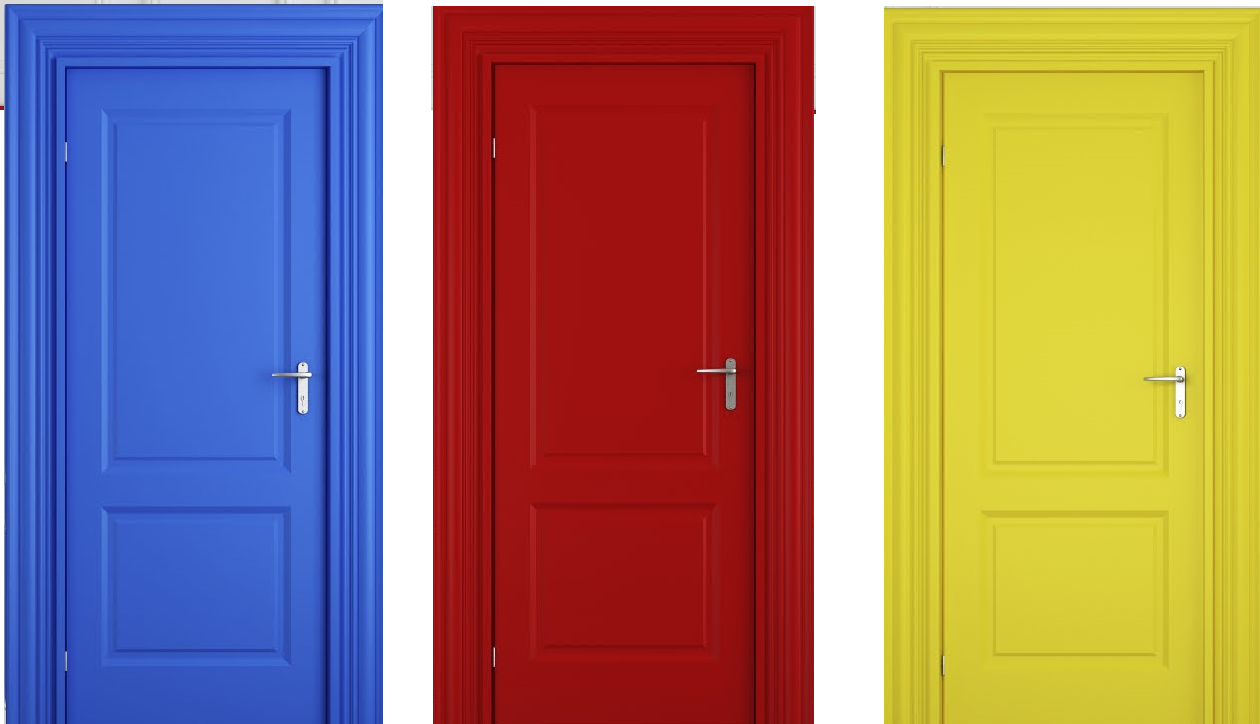
\includegraphics[width=\textwidth]{Zarta_Vrata_brez.png}

\end{figure}
\note{Začnimo najprej z vprašanjem. Pred vami so postavljena 3 vrata. Za enimi je nagrada ki jo želite (npr. lep nov avto). Za drugima dvema pa stojita dve kozi. }
\end{frame}

\begin{frame}
  \begin{figure}
  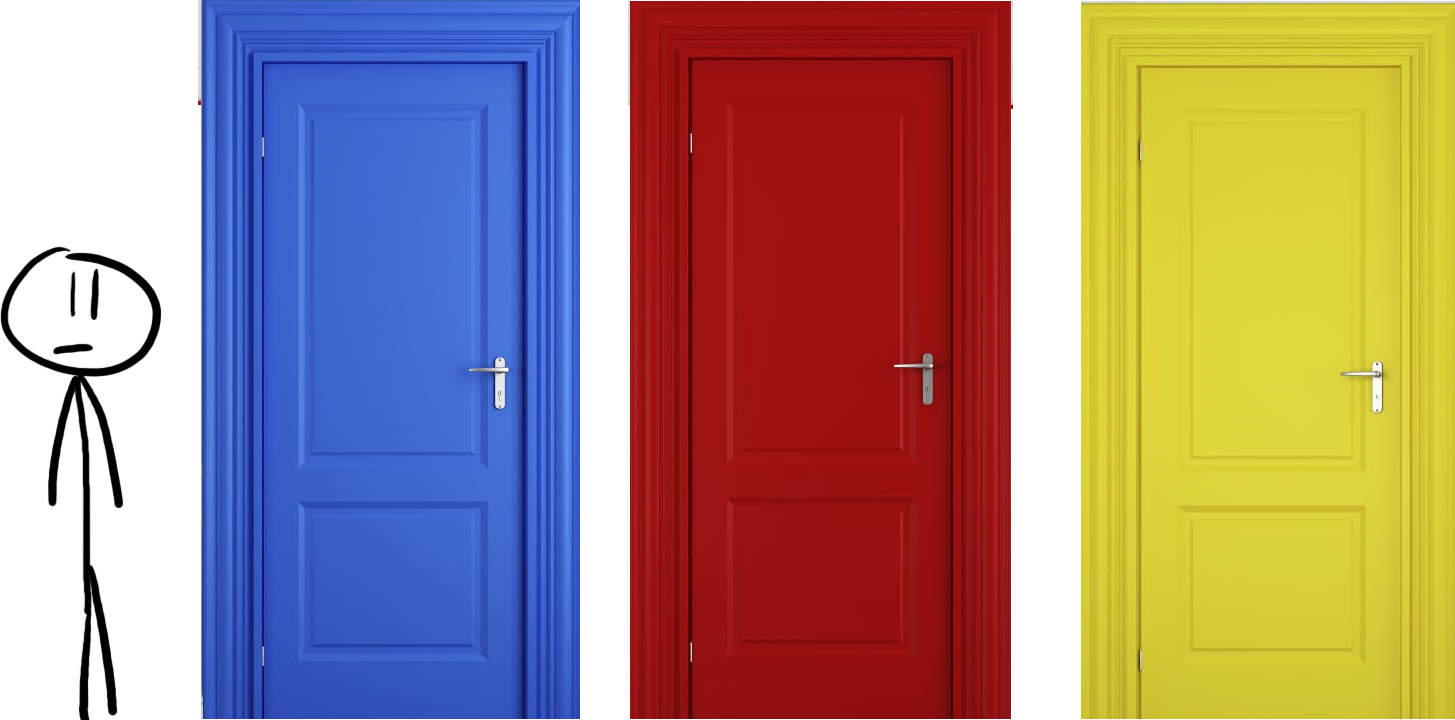
\includegraphics[width=\textwidth]{Izbira_vrat.png}
  \end{figure}
\note{Recimo da izberemo prva vrata }
\end{frame}
\begin{frame}
  \begin{figure}
  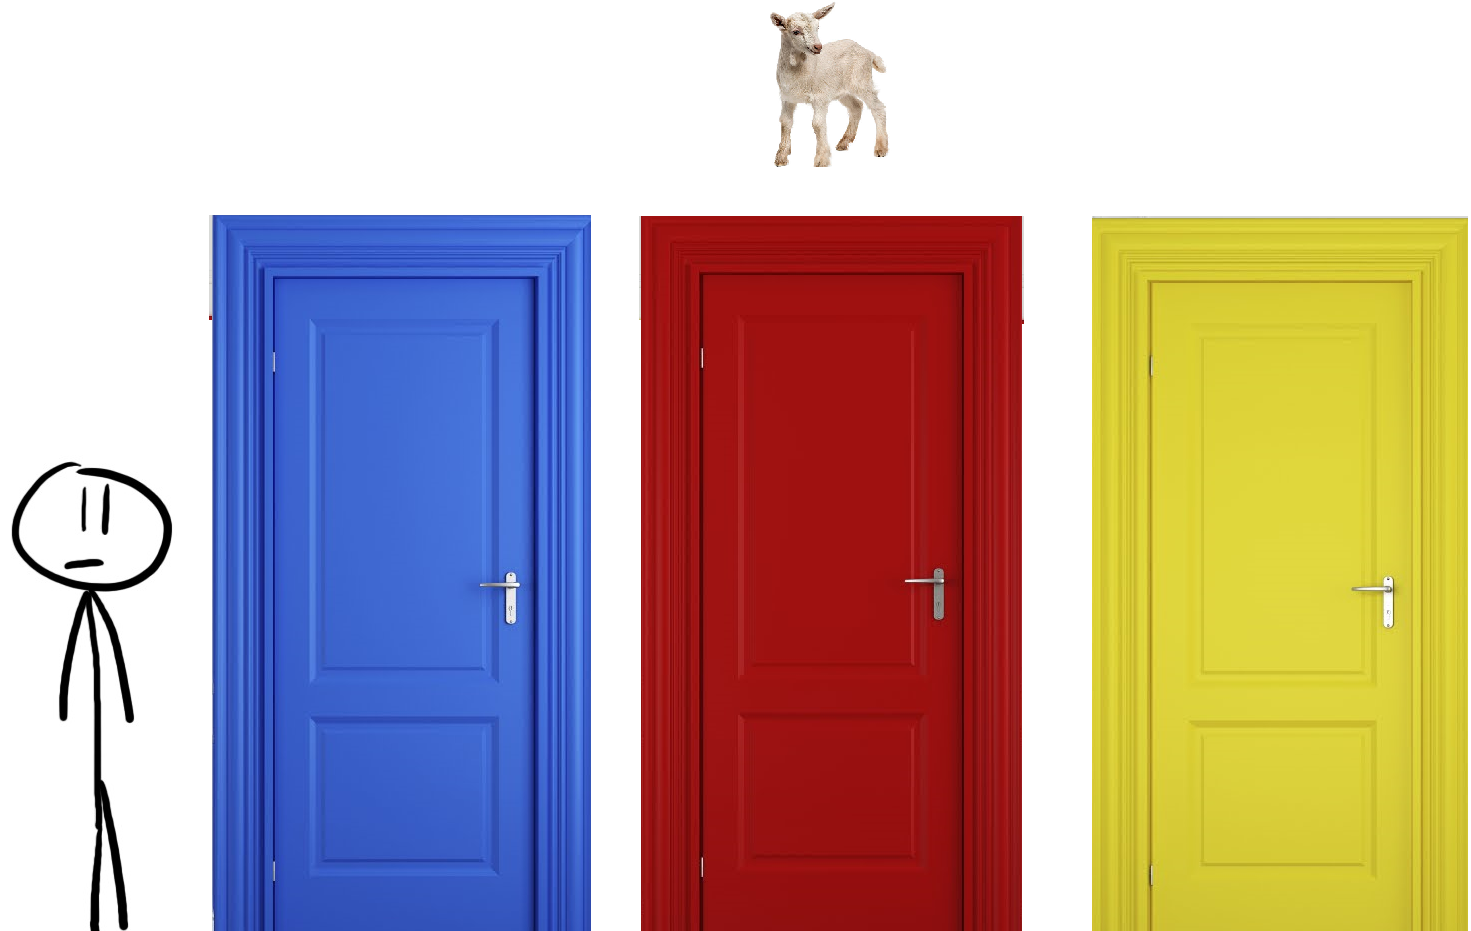
\includegraphics[width=\textwidth]{Izbira_vrat_2.png}
  \end{figure}
\note{Sedaj jaz odprem eno od preostalih dveh vrat ki vsebuje kozo (vemo da so vsaj ena vrata taka ). Brez škode za splošnost naj bodo to druga vrata. Kolikšna je sedaj verjetnost da je avto za vašimi vrati? The answer will shock you}
\end{frame}

\begin{frame}
  \begin{figure}
  
\includegraphics[width=\textwidth]{LetsMakeADeal.jpg}
  \end{figure}
\note{Najprej malo zgodovine. Let's make a deal je bila ameriška televizijska oddaja kjer so tekmovalci bili postaljeni pred tremi vratami, za enimi je bil avto za drugima dvema pa koza. tekmovalci so izbrali poljubna vrata nato pa je Monty  odprl ena vrata za katerim je bila koza. Nato je Monty tekmovalcem dal priložnost, da pri svoji izbiri  ostanejo, ali pa zamenjajo na druga ,še neodprta, vrata. The Monty Hall problem nas sprašuje, kdaj imamo največjo možnost zmage, če pri svoji izbiri ostanemo, vrata zamenjamo ali je pa  to od izida to čisto vseeno   }
\end{frame}
\begin{frame}
  \begin{table}[]
        \centering


    \begin{tabular}{|c|c|c|}
    \hline
    \multicolumn{1}{|l|}{Vrata 1} & \multicolumn{1}{l|}{Vrata 2 } & Vrata 3 \\ \hline
                      $C$     & $G_{2}$                      &$G_{1}$  \\
                        $C$   &   $G_{1}$                    & $G_{2}$ \\
                     $G_{1}$       &        $C$                   & $G_{2}$ \\
                       $G_{1}$      &                $G_{2}$       &  $C$    \\
                         $G_{2}$      &       $G_{1}$                  & $C$ \\
                              $G_{2}$       &  $C$               &  $G_{1}$   \\\hline
    \end{tabular}
    \end{table}
  \note{Probajmo ta primer najprej rešiti s tabelo. Privzemimo da vedno izbereo prvo možnost in poglejo kolikokrat zmagamo ,... neda se mi pisat }
\end{frame}

\begin{frame}
  $P(A)=\text{Monty odpre vrata 2}$\\
  $P(B)=\text{avto je za vrati 1}$
  $$P(A)P(B/A)=P(AB)=P(B)P(A/B)$$

\end{frame}
\begin{frame}
    $P(A)=\text{Monty odpre vrata 2}$\\
    $P(B)=\text{avto je za vrati 1}$
    $$P(B/A)=P(A/B)\frac{P(B)}{P(A)}$$
\end{frame}
\begin{frame}
    $P(A)=\text{Monty odpre vrata 2}$\\
    $P(B)=\text{avto je za vrati 1}$
    $$P(B/A)=\underbrace{P(A/B)}_{\frac{1}{2}}\frac{\overbrace {P(B)}^{\frac{1}{3}}}{\underbrace{P(A)}_{\frac{1}{2}}}$$
\end{frame}
\title{Bernard's Paradox}
\begin{frame}
  \maketitle
\end{frame}
\begin{frame}
  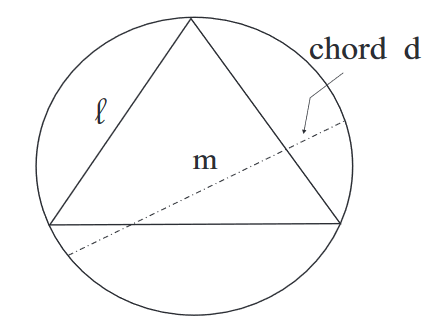
\includegraphics[width=\textwidth]{Bernard_1.png}
\end{frame}
\begin{frame}
  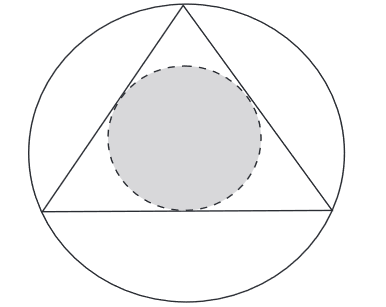
\includegraphics[width=\textwidth]{Bernard_2.png}
\end{frame}
\begin{frame}
  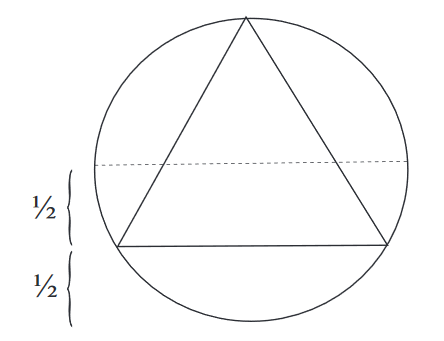
\includegraphics[width=\textwidth]{Bernard_3.png}
\end{frame}
\begin{frame}
  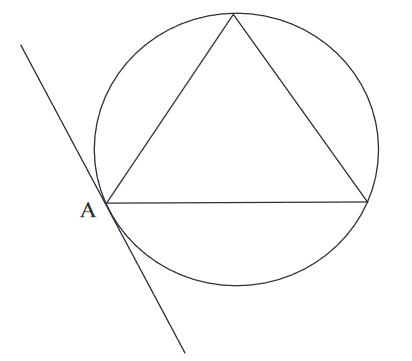
\includegraphics[width=\textwidth]{Bernard_4.png}
\end{frame}
\begin{frame}
  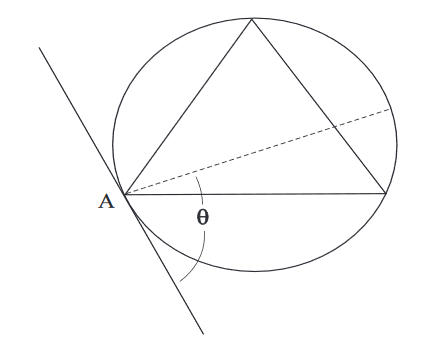
\includegraphics[width=\textwidth]{Bernard_5.png}
\end{frame}

\end{document}
